\documentclass[Lecture.tex]{subfiles}
\begin{document}
\section{5.1: Distance and Accumulated Change}

\subsection{Constant Functions}
\begin{frame}{Constant Functions}
  \only<1-5>{Suppose a car is traveling at 60 miles per hour for 2 hours.
    \onslide<2->{How far did the car go?}\\}
  \vfill
  \begin{minipage}[t]{\linewidth}
    \only<3-5>{
      This is easy:
      $$\onslide<4-5>{60\ \frac{\text{miles}}{\text{hour}} \cdot 2\ \text{hours} =} \onslide<5>{120\ \text{miles}.}$$
    }
    \only<6-7>{
      Geometrically, this is the area under the constant curve $y(t) = 60$ between $t = 0$ and $t = 2$:
      \onslide<7>{\begin{center}
          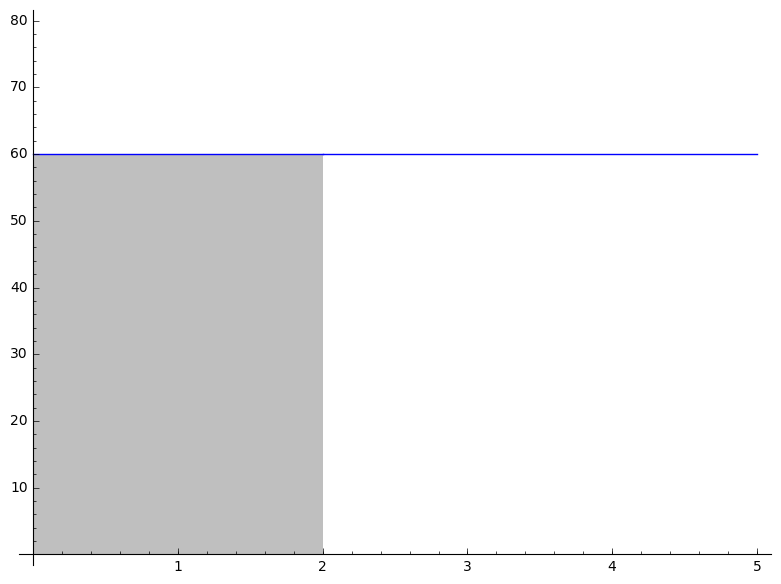
\includegraphics[scale=0.25]{constantVelocity}
      \end{center}}
    }
    \only<8>{
      This says that under constant velocity, $v$, the position of the car, $s(t)$, relative to the starting point at time $0 \leq t$ is just
      $$s(t) = v \cdot t.$$
    }
  \end{minipage}
\end{frame}

\subsection{Linear Functions}
\begin{frame}{Linear Functions}
  \only<1-3>{According to Car and Driver, a 2006 Bugatti Veyron is capable of an acceleration of $11.59 \operatorname{m}/\operatorname{s}^2$.
    Assume the car starts at rest and accelerates at this constant rate.\\}

  \vfill
  
  \begin{minipage}[t]{\linewidth}
    \only<2-3>{
      By the observation in the last example, we can compute the velocity at time $t$ as the area under the constant curve $y(t) = 11.59$:
      \onslide<3>{
        \begin{center}
          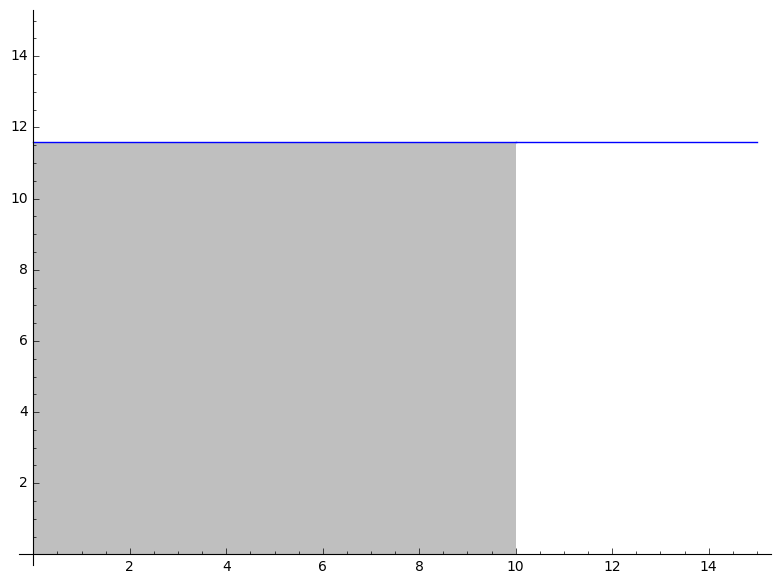
\includegraphics[scale=0.25]{constantAcceleration}
        \end{center}
      }
    }
    \only<4-5>{
      The velocity is linear: $v(t) = 11.59\cdot t$.
      Hence the position, $s(t)$, is the area under the velocity curve:
      \onslide<5->{
        \begin{center}
          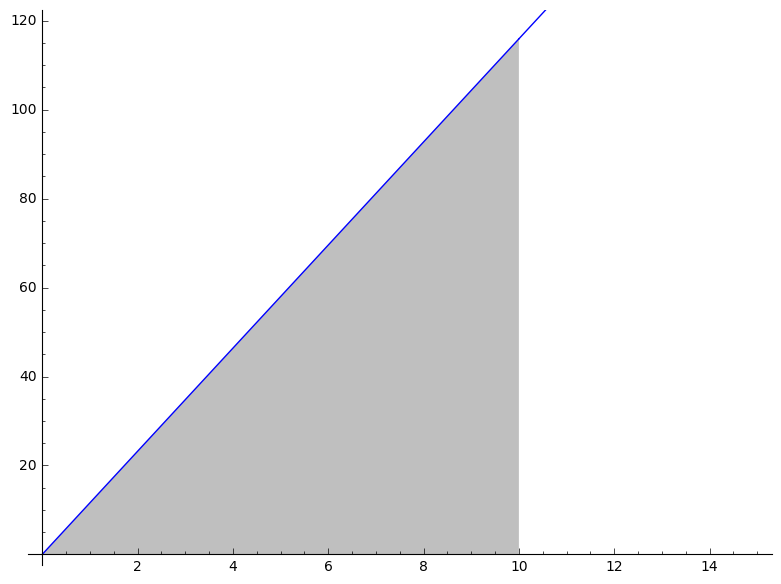
\includegraphics[scale=0.25]{linearVelocity}
        \end{center}
      }
    }
    \only<6->{
      Therefore the position at time $t$ is:
      \begin{eqnarray*}
        \onslide<7->{s(t) &=&} \onslide<8->{\frac{1}{2}v(t)\cdot t\\} 
        \onslide<9->{ &=& \frac{1}{2}(11.59 \cdot t)\cdot t\\}
        \onslide<10->{ &=& \frac{11.59}{2}t^2.}
      \end{eqnarray*}
    }
  \end{minipage}
\end{frame}

\subsection{Non-Linear Functions}
\begin{frame}{Non-Linear Functions}
  \only<1-12>{What happens when the area is not a nice geometric object?\\}
  \vfill
  \begin{minipage}[t]{\linewidth}
    \only<2-9>{
      Can we tell how far a car traveled if we are given the following table of times and velocities?
      \onslide<3->{
        \begin{center}
          \begin{tabular}{c||c|c|c|c|c|c}
            time (sec) & 0 & 2 & 4 & 6 & 8 & 10\\
            \hline
            speed (ft/sec) & 20 & 30 & 38 & 44 & 48 & 50\\
          \end{tabular}
        \end{center}
      }
      \onslide<4->{This is clearly not linear:}
      \onslide<5->{
        $$\onslide<5->{\frac{30 - 20}{2 - 0} =} \onslide<6->{5}\onslide<7->{\ \text{and}\ }\onslide<8->{\frac{50-48}{10-8}}\onslide<9->{ = 1.}$$
      }
    }
    \only<10-12>{
      We can fit a curve to these points:
      \onslide<11-12>{
        \begin{center}
          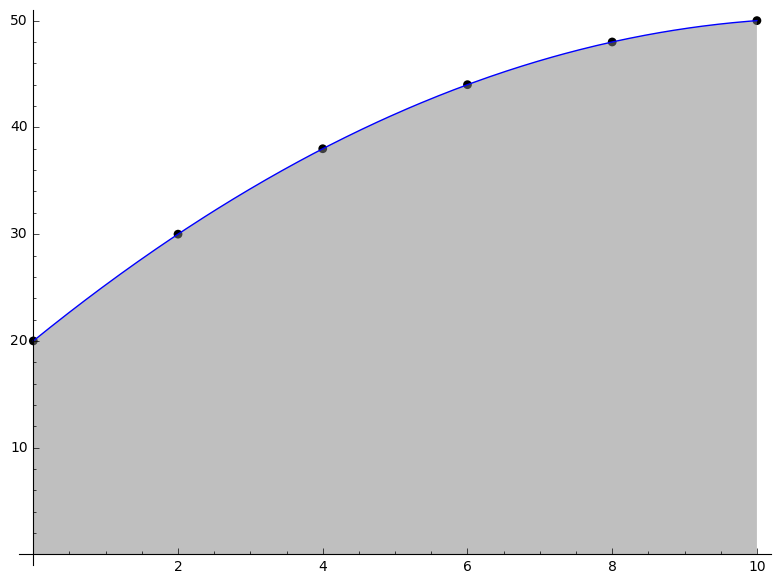
\includegraphics[scale=0.3]{nonlinearVelocity}
        \end{center}
      }
      \onslide<12>{How do we compute the area of the shaded region?}
    }
    \only<13-16>{
      We could assume constant velocity between the two points and estimate.
      \onslide<14->{Say we assume the velocity is the velocity at the left endpoint:}
      \onslide<15->{
        \begin{center}
          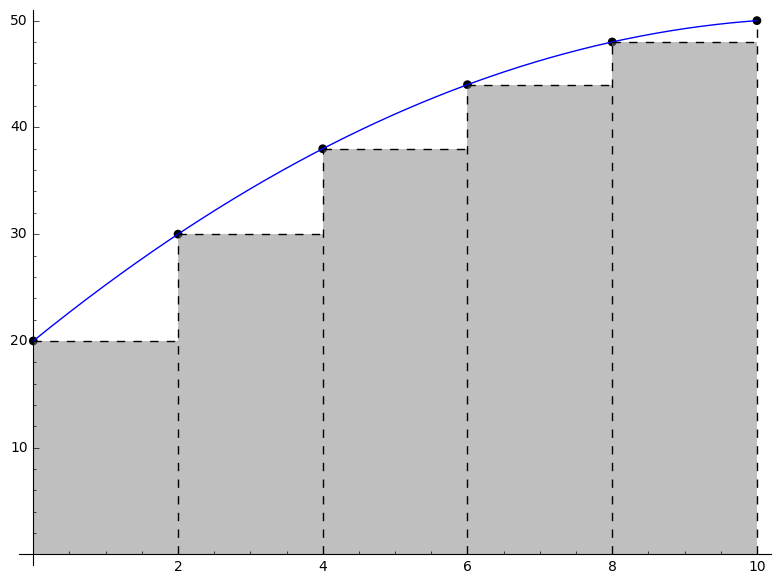
\includegraphics[scale=0.3]{nonlinearLeftSum}
        \end{center}
      }
      \onslide<16->{This is an underestimate of the area.}
    }
    \only<17-22>{
      \begin{center}
        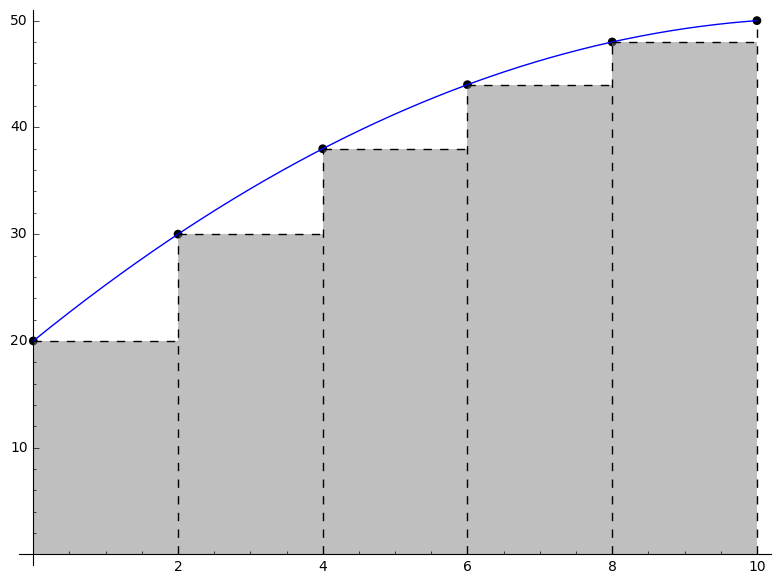
\includegraphics[scale=0.2]{nonlinearLeftSum}
      \end{center}
      
      \begin{itemize}
      \item<17->
        Each rectangle has width 2.
      \item<18->
        The height of each rectangle is the height of the left endpoint.
      \item<19->
        Our area estimate is:
        \begin{eqnarray*}
          \onslide<20->{2(20 + 30 + 38 + 44 + 48) &=&}
          \onslide<21->{2(180)\\}
          \onslide<22->{&=& 360\ \text{feet}.}
        \end{eqnarray*}
      \end{itemize}
    }
    \only<23-25>{
      We could also assume the velocity is the velocity at the right endpoint:
      \onslide<24->{
        \begin{center}
          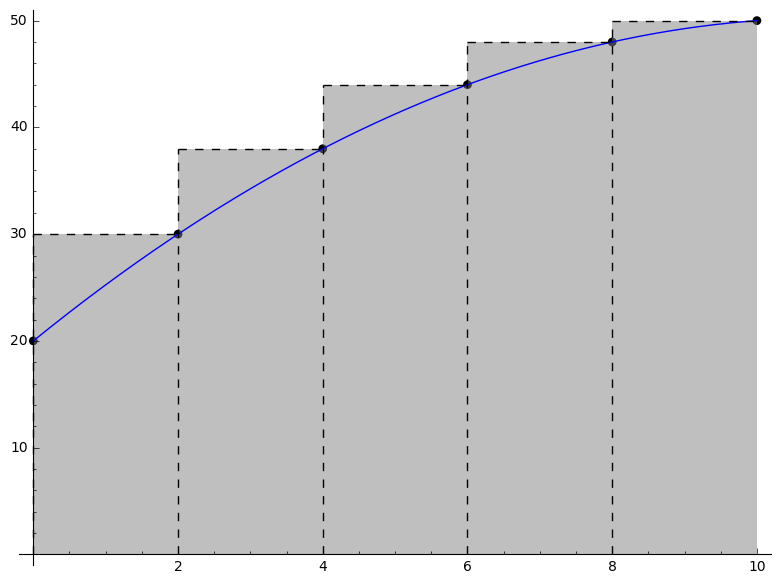
\includegraphics[scale=0.3]{nonlinearRightSum}
        \end{center}
      }
      \onslide<25->{This is an overestimate of the area.}
    }
    \only<26-31>{
      \begin{center}
        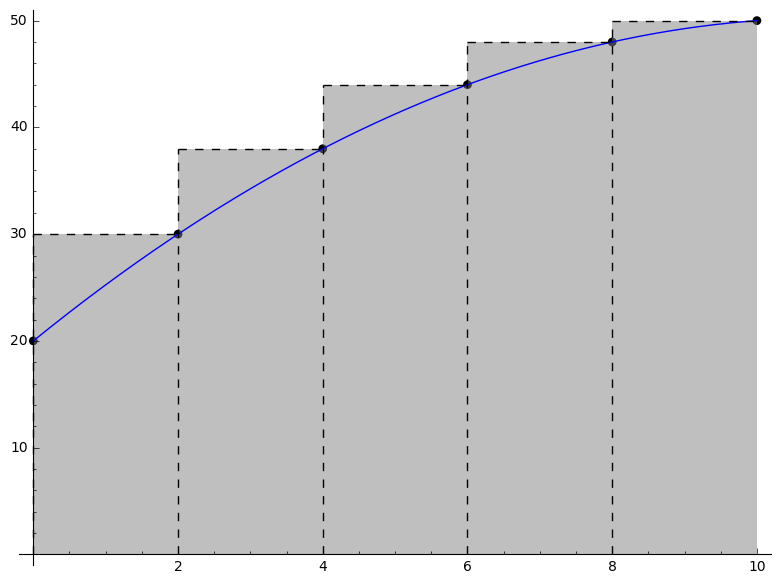
\includegraphics[scale=0.2]{nonlinearRightSum}
      \end{center}
      \begin{itemize}
      \item<26->
        Each rectangle has width 2.
      \item<27->
        The height of each rectangle is the height of the right endpoint.
      \item<28->
        Our area estimate is:
        \begin{eqnarray*}
          \onslide<29->{2(30 + 38 + 44 + 48 + 50) &=&}
          \onslide<30->{2(210)\\}
          \onslide<31->{&=& 420\ \text{feet}.}
        \end{eqnarray*}
      \end{itemize}
    }
    \only<31->{
      This tells us:
      \begin{itemize}
      \item<32->
        The distance traveled is {\bf at least} 360 feet.
      \item<33->
        The distance traveled is {\bf at most} 420 feet.
      \item<34->
        The distance traveled must be somewhere between these two.
      \item<35->
        The average of these estimates is 
        $$\frac{420 + 360}{2} = 390$$
        feet, which gives a better estimate.
      \end{itemize}
      \onslide<36->{Can we do better?}
      \onslide<37->{If so, how?}
    }
  \end{minipage}
\end{frame}

\subsection{Right Endpoint Estimates}
\begin{frame}{Right Endpoint Estimates}
  We'll use the old linear velocity example, $v(t) = 11.59t$, to analyse these methods:
  \onslide<2->{
    \begin{center}
      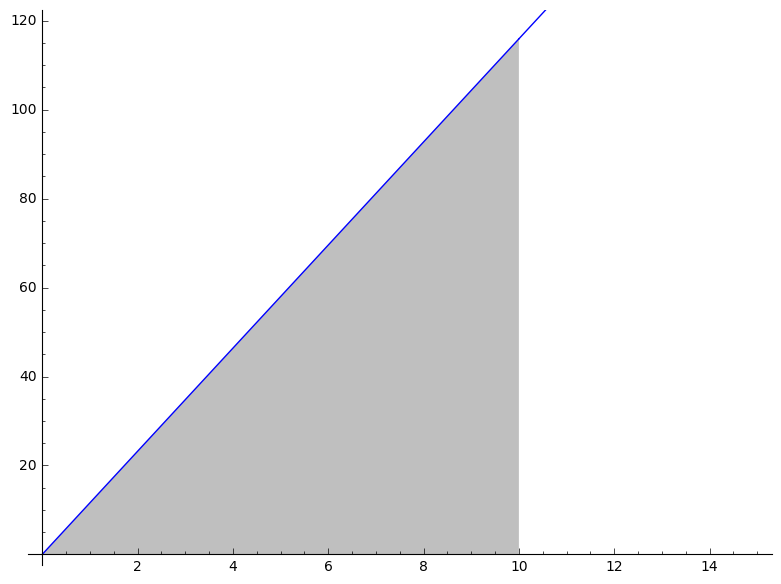
\includegraphics[scale=0.3]{linearVelocity.png}
    \end{center}
  }
\end{frame}

\begin{frame}{Right Endpoint Estimate}
  Say we use the two points $t = 0$ and $t = 10$.
  \onslide<2->{We know the area under the curve is given by:
    \onslide<3->{$$\frac{1}{2}v(t)\cdot t.$$}
  }
  \onslide<4->{
    Our estimate is quite bad:\\
    \begin{minipage}{.48\linewidth}
      \onslide<5->{
        \begin{center}
          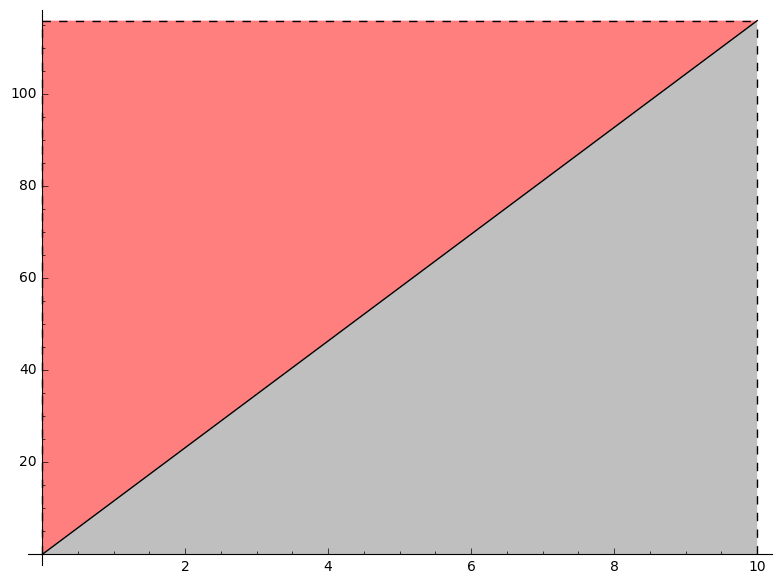
\includegraphics[scale=0.25]{rightEst1Pt}
      \end{center}}
    \end{minipage}
    \hfill
    \begin{minipage}{.48\linewidth}
      \begin{itemize}
      \item<6->
        Red is the error.
      \item<7->
        Grey is the area.
      \item<8->
        The estimate for the area is the sum of the red and grey areas.
      \item<9->
        The error is equal to the actual area!
      \end{itemize}
    \end{minipage}
  }
\end{frame}

\begin{frame}{Three Equidistant Points}
  If we try three equidistant points, 0, $\frac{t}{2}$, and $t$, then we get:\\
  \vfill
  \begin{minipage}{0.48\linewidth}
    \onslide<2->{
      \begin{center}
        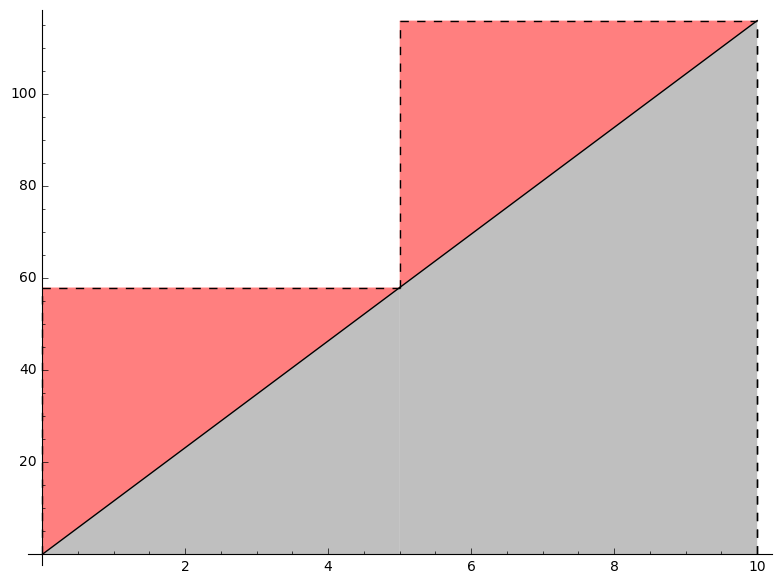
\includegraphics[scale=0.25]{rightEst2Pts}
      \end{center}
    }
  \end{minipage}
  \hfill
  \begin{minipage}{0.48\linewidth}
    \begin{itemize}
    \item<3->
      Visibly, this is a better estimate.
    \item<4->
      The error is the area of the two red triangles.
    \item<5->
      Both have base length $\frac{t}{2}$; here $t = 10$.
    \item<6->
      The height of the left triangle is $v\left(\frac{t}{2}\right)$.
    \item<7->
      The height of the right triangle is $v(t) - v\left(\frac{t}{2}\right)$.
    \end{itemize}
  \end{minipage}
\end{frame}

\begin{frame}{Three Equidistant Points (Cont.)}
  So, the total error is:\\
  \onslide<2->{
    \scalebox{.75}{\parbox{\linewidth}{
        \begin{eqnarray*}
          \onslide<2->{\frac{1}{2}\left[v(t) - v\left(\frac{t}{2}\right)\right]\frac{t}{2} +}
          \onslide<3->{\frac{1}{2}v\left(\frac{t}{2}\right)\cdot\frac{t}{2}}
          \onslide<4->{&=&\frac{1}{2}\left[v(t) - v\left(\frac{t}{2}\right) + v\left(\frac{t}{2}\right)\right]\frac{t}{2}\\}
          \onslide<5->{&=& \frac{1}{2}\left(\frac{1}{2}v(t)\cdot t\right).}
        \end{eqnarray*}
    }}\\
  }
  \onslide<6->{By adding one more point, we've reduced the error by a factor of two!}
\end{frame}

\begin{frame}{Four Equidistant  Points (Cont.)}
  If we try four equidistant points, 0, $\frac{t}{3}$, $\frac{2t}{3}$, and $t$, then we get:\\
  \vfill
  \begin{minipage}{0.48\linewidth}
    \onslide<2->{
      \begin{center}
        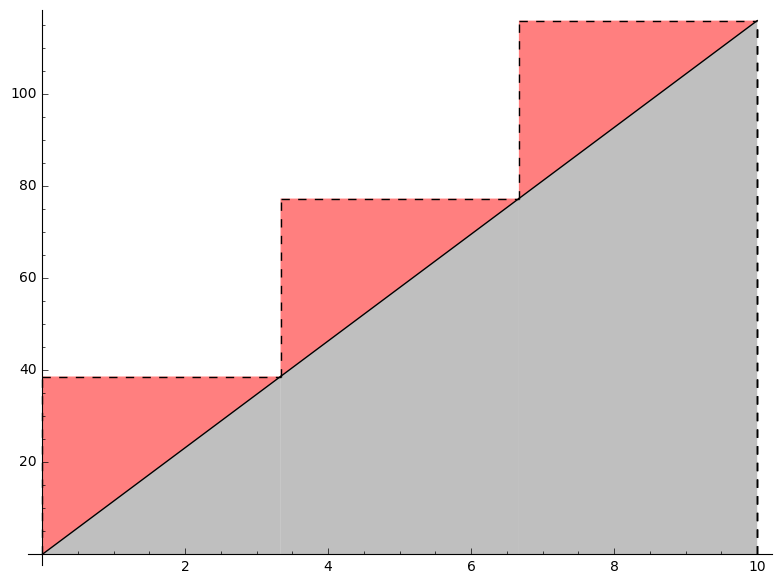
\includegraphics[scale=0.25]{rightEst3Pts}
      \end{center}
    }
  \end{minipage}
  \hfill
  \begin{minipage}{0.48\linewidth}
    \begin{itemize}
    \item<3->
      Visibly, this is an even better estimate.
    \item<4->
      All three red triangles have base length $\frac{t}{3}$.
    \item<5->
      The height of the left triangle is $v\left(\frac{t}{3}\right)$.
    \item<6->
      The height of the middle triangle is $v\left(\frac{2t}{3}\right) - v\left(\frac{t}{3}\right)$.
    \item<7->
      The height of the right triangle is $v(t) - v\left(\frac{2t}{3}\right)$.
    \end{itemize}
  \end{minipage}
\end{frame}

\begin{frame}{Four Equidistant Points (Cont.)}
  So, the total error is:\\
  \onslide<2->{
    \scalebox{.5}{\parbox{\linewidth}{
        \begin{eqnarray*}
          \onslide<2->{\frac{1}{2}\left[v(t) - v\left(\frac{2t}{3}\right)\right]\frac{t}{3} +}
          \onslide<3->{\frac{1}{2}\left[v\left(\frac{2t}{3}\right) - v\left(\frac{t}{3}\right)\right]\frac{t}{2} + }
          \onslide<4->{\frac{1}{2}v\left(\frac{t}{3}\right)\frac{t}{3}}
          \onslide<5->{&=&
            \frac{1}{2}
            \left[
              v(t) - v\left(\frac{2t}{3}\right) + 
              v\left(\frac{2t}{3}\right) \right.
              - \left.
              v\left(\frac{t}{3}\right) + 
              v\left(\frac{t}{3}\right)
              \right]
            \frac{t}{3}\\}
          \onslide<6->{&=& \frac{1}{3}\left(\frac{1}{2}v(t)\cdot t\right).}
        \end{eqnarray*}
    }}\\
  }
  \onslide<7->{By using four points, we've reduced the initial error by a factor of three!}
\end{frame}

\begin{frame}{$n+1$ Equidistant Points}
  If we use $n+1$ equidistant points,
  \onslide<2->{
    $$\onslide<2->{t_0 = 0,\,}
    \onslide<3->{t_1 = \frac{t}{n},\,}
    \onslide<4->{t_2 = \frac{2t}{n},\,}
    \onslide<5->{\ldots,\,}
    \onslide<6->{t_{n-1} = \frac{(n-1)t}{n},\,}
    \onslide<7->{t_n = t,}$$}
  \onslide<8->{then we expect the error will be sum of the areas of $n$ triangles.}
  \onslide<9->{The $k^\text{th}$ triangle, for $1 < k < n$, has: }
  \begin{itemize}
  \item<10->
    base length $\frac{t}{n}$,
  \item<11->
    height $v(t_k) - v(t_{k-1})$,
  \item<12->
    area 
    $$\frac{1}{2}\left[v\left(t_k\right) - v\left(t_{k-1}\right)\right]\frac{t}{n}$$
  \end{itemize}
  \onslide<13->{
    \begin{rmk}
      Note that $v(t_0) = v(0) = 0$.
    \end{rmk}
  }
\end{frame}

\begin{frame}{$n+1$ Equidistant Points}
  Adding up the areas of each of the triangles, we get the total error:\\
  \scalebox{.65}{\parbox{.9\linewidth}{
      \begin{eqnarray*}
        \onslide<2->{
          \frac{1}{2}\left[
          }
          \onslide<3->{
            v(t) - v(t_{k-1}) +
          }
          \onslide<4->{
            v(t_{k-1}) - v(t_{k-2}) +
          }
          \onslide<5->{
            \ldots +
          }
          \onslide<6->{
            v(t_2) - v(t_1) +
          }
          \onslide<7->{
            v(t_1) - v(t_0)\right]
        }
        \onslide<8->{
          \frac{t}{n}
        }
        \onslide<9->{
          &=& \frac{1}{2}v(t)\cdot\frac{t}{n}\\
        }
        \onslide<10->{
          &=& \frac{1}{n}\left(\frac{1}{2}v(t)\cdot t\right).
        }
      \end{eqnarray*}
  }}\\
  \onslide<11->{
    Therefore, if we use $n+1$ equidistant points, we have overestimated the area under $v(t)$ by
    $$\frac{1}{n}\left(\frac{1}{2}v(t)\cdot t\right).$$
  }
\end{frame}

\subsection{Left Endpoint Estimates}
\begin{frame}{Left Estimate}
  The situation for a left endpoint estimate is symmetric:
  \vfill
  \begin{minipage}{\linewidth}
    \only<2-3>{
      2 Equidistant Points:
      \begin{center}
        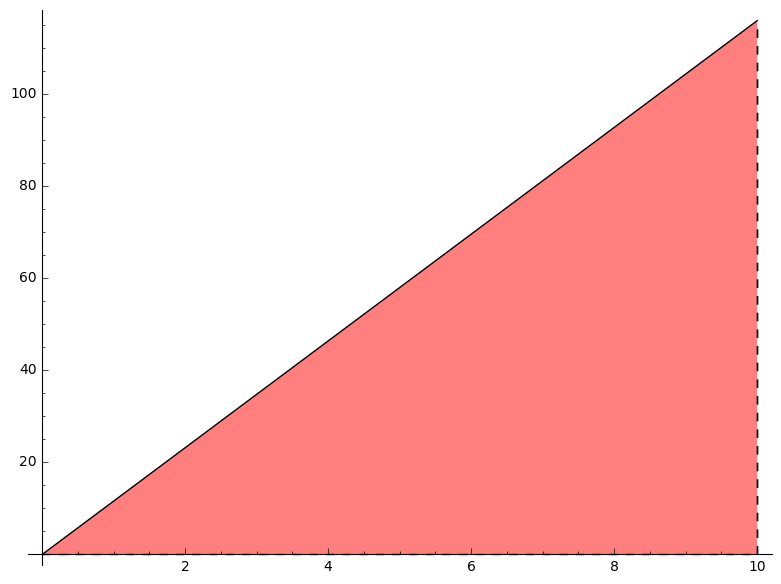
\includegraphics[scale=0.3]{leftEst1Pt}
      \end{center}
      \only<3>{Our Estimate for the area here is {\bf zero}.
        We have {\bf underestimated} the area by $\frac{1}{2}v(t)\cdot t$.}
    }
    \only<4-5>{
      3 Equidistant Points:
      \begin{center}
        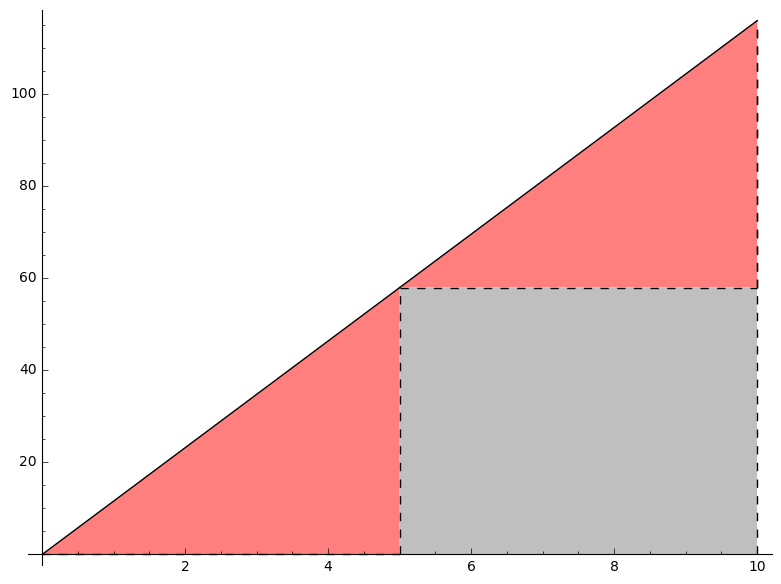
\includegraphics[scale=0.3]{leftEst2Pts}
      \end{center}
      \only<5>{We have {\bf underestimated} the area by $\frac{1}{2}\left(\frac{1}{2}v(t)\cdot t\right)$.}
    }
    \only<6-7>{
      4 Equidistant Points:
      \begin{center}
        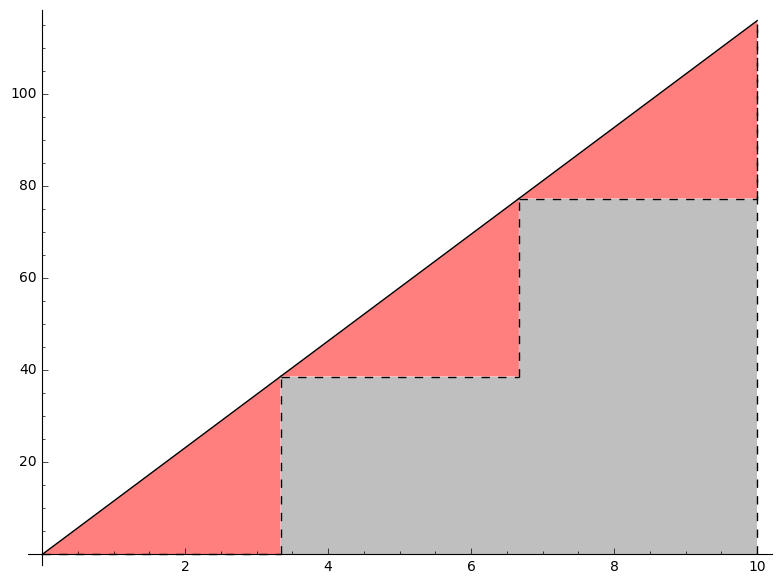
\includegraphics[scale=0.3]{leftEst3Pts}
      \end{center}
      \only<7>{We have {\bf underestimated} the area by $\frac{1}{3}\left(\frac{1}{2}v(t)\cdot t\right)$.}
    }
  \end{minipage}
\end{frame}

\begin{frame}{Left Estimate}
  By the same analysis as with the right estimates, using $n+1$ equidistant points
  \onslide<2->{
    $$\onslide<2->{t_0 = 0,\,}
    \onslide<3->{t_1 = \frac{t}{n},\,}
    \onslide<4->{t_2 = \frac{2t}{n},\,}
    \onslide<5->{\ldots,\,}
    \onslide<6->{t_{n-1} = \frac{(n-1)t}{n},\,}
    \onslide<7->{t_n = t,}$$}
  \onslide<8->{then we expect the error will be sum of the areas of $n$ triangles.}
  \onslide<9->{The $k^\text{th}$ triangle, for $1 < k < n$, has: }
  \begin{itemize}
  \item<10->
    base length $\frac{t}{n}$,
  \item<11->
    height $v(t_k) - v(t_{k-1})$,
  \item<12->
    area 
    $$\frac{1}{2}\left[v\left(t_k\right) - v\left(t_{k-1}\right)\right]\frac{t}{n}$$
  \end{itemize}
  \onslide<13->{
    \begin{rmk}
      Note that $v(t_0) = v(0) = 0$.
    \end{rmk}
  }
\end{frame}

\begin{frame}{$n+1$ Equidistant Points}
  Adding up the areas of each of the triangles, we get the total error:\\
  \scalebox{.65}{\parbox{.9\linewidth}{
      \begin{eqnarray*}
        \onslide<2->{
          \frac{1}{2}\left[
          }
          \onslide<3->{
            v(t) - v(t_{k-1}) +
          }
          \onslide<4->{
            v(t_{k-1}) - v(t_{k-2}) +
          }
          \onslide<5->{
            \ldots +
          }
          \onslide<6->{
            v(t_2) - v(t_1) +
          }
          \onslide<7->{
            v(t_1) - v(t_0)\right]
        }
        \onslide<8->{
          \frac{t}{n}
        }
        \onslide<9->{
          &=& \frac{1}{2}v(t)\cdot\frac{t}{n}\\
        }
        \onslide<10->{
          &=& \frac{1}{n}\left(\frac{1}{2}v(t)\cdot t\right).
        }
      \end{eqnarray*}
  }}\\
  \onslide<11->{
    Therefore, if we use $n+1$ equidistant points, we have {\bf underestimated} the area under $v(t)$ by
    $$\frac{1}{n}\left(\frac{1}{2}v(t)\cdot t\right).$$
  }  
\end{frame}

\begin{frame}{More Is Better}
  \begin{itemize}
  \item<1->
    Using $n+1$ points for either a left or a right estimate, the absolute value of the error in estimating the area under the curve between $0$ and $t = 10$ is given by 
    $$\frac{1}{n}\left(\frac{1}{2}v(t) \cdot t \right) = \frac{1}{n}\left(\frac{11.59}{2}100\right).$$
  \item<2->
    This tells us that as $n$ becomes large, the error decreases.
    That is, the more points, the better the estimate!
  \item<3->
    As $n$ grows larger, the right estimate {\bf decreases} towards the actual area and the left estimate {\bf increases} towards the actual area.
  \end{itemize}
\end{frame}

\begin{frame}{Right Error}
  \animategraphics[loop,controls,scale=0.3]{12}{errorRight/errorRight-}{0}{99}
\end{frame}

\begin{frame}{Left Error}
  \animategraphics[loop,controls,scale=0.3]{12}{errorLeft/errorLeft-}{0}{99}
\end{frame}

\subsection{Partitions}
\begin{frame}{Partitions of an Interval}
  To generalize our methods to non-linear curves, we introduce some notation.
  \begin{defn}
    For a continuous function, $f$, on an interval $[a,b]$, a set of $n+1$ equidistant points,
    $$t_0 = a < t_1 < t_2 < \ldots < t_{n-1} < t_n = b$$
    is called a {\it partition} of $[a,b]$.
  \end{defn}
\end{frame}

\begin{frame}{Partitions and Estimates}
  These $n+1$ points are called a partition because they partition $[a,b]$ into $n$ smaller intervals of length $\Delta t$
  \begin{center}
    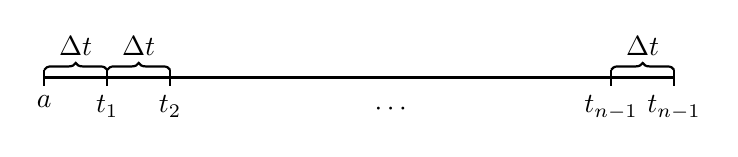
\begin{tikzpicture}[xscale=8]
      \draw[-][very thick] (0,0) -- (.1,0);
      \draw[-][very thick] (.1,0) -- (.2,0);
      \draw[-][very thick] (.2,0) -- (.9,0);
      \draw[-][very thick] (.9,0) -- (1,0);
      \draw [
        thick,
        decoration={
          brace,
          raise=0.1cm
        },
        decorate
      ]
      (0,0) -- (.1,0) node[pos=0.5,anchor=north,yshift=.65cm]{$\Delta t$};
      \draw [
        thick,
        decoration={
          brace,
          raise=0.1cm
        },
        decorate
      ]
      (.1,0) -- (.2,0) node[pos=0.5,anchor=north,yshift=.65cm]{$\Delta t$};
      \draw [
        thick,
        decoration={
          brace,
          raise=0.1cm
        },
        decorate
      ]
      (.9,0) -- (1,0) node[pos=0.5,anchor=north,yshift=.65cm]{$\Delta t$};
      \draw [thick] (0,-.1) node[below]{$a$} -- (0,0.1);
      \draw [thick] (.1,-.1) node[below]{$t_1 $} -- (.1,0.1);
      \draw [thick] (.2,-.1) node[below]{$t_2 $} -- (.2,0.1);
      \draw [thick] (.9,-.1) node[below]{$t_{n-1}$} -- (.9,0.1);
      \draw [thick] (1,-.1) node[below]{$t_{n-1}$} -- (1,0.1);
      \node[align=center,below] at (.55,-.2){$\cdots$};
    \end{tikzpicture}
  \end{center}
  where 
  $$\Delta t = \frac{b - a}{n}.$$
  
  \onslide<2->{
    These $n$ smaller intervals form the bases of the rectangles we use to estimate the area under a curve.
  }
\end{frame}

\subsection{Left- and Right-Hand Sums}

\begin{frame}{Sums}
  \begin{defn}
    Let $f$ be a continuous function on the interval $[a,b]$.
    \onslide<2->{Given a partition
      $$a = t_0 < t_1 < \cdots < t_{n-1} < t_n = b$$}
    \begin{itemize}
    \item<3->
      The {\it Left-Hand Sum} is
      $$f(t_0)\Delta t + f(t_1)\Delta t + \cdots + f(t_{n-2})\Delta t + f(t_{n - 1})\Delta t.$$
    \item<4->
      The {\it Right-Hand Sum} is
      $$f(t_1)\Delta t + f(t_2)\Delta t + \cdots + f(t_{n-1})\Delta t + f(t_n)\Delta t.$$
    \end{itemize}
  \end{defn}
\end{frame}

\begin{frame}{Sums (Cont.)}
  \only<1>{
    The Left-Hand Sum underestimates the area under the curve:
    \begin{center}
      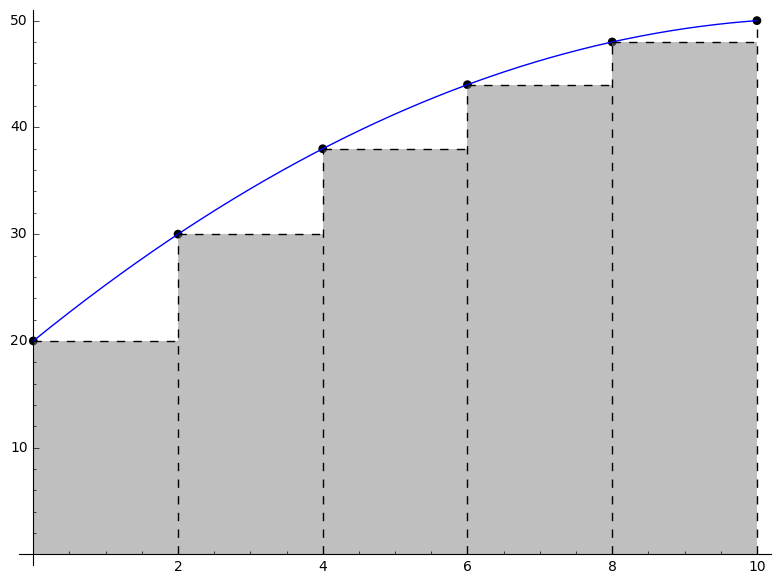
\includegraphics[scale=0.3]{nonlinearLeftSum}
    \end{center}
  }
  \only<2>{
    The Right-Hand Sum overestimates the area under the curve:
    \begin{center}
      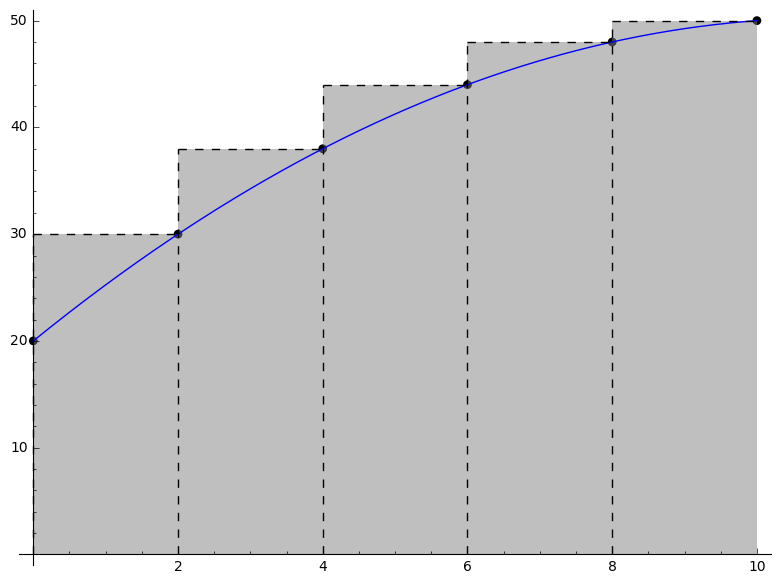
\includegraphics[scale=0.3]{nonlinearRightSum}
    \end{center}
  }
\end{frame}

\begin{frame}{Sigma Notation}
  For ease of notation, we write the left-hand sum as
  \onslide<2->{
    $$\sum_{i = 0}^{n-1} f(t_i)\Delta t = f(t_0)\Delta t + \ldots + f(t_{n-1})\Delta t$$
  }
  \onslide<3->{
    and we write the right-hand sum as
    $$\sum_{i = 1}^n f(t_i)\Delta t = f(t_1)\Delta t + \ldots + f(t_n)\Delta t.$$
  }
  \onslide<4->{
    The letter $i$ is the {\it index} of the summation and the letter $n$ is the {\it upper bound} of the summation.
    The $i = 0$ underneath the sigma, $\Sigma$, indicates the sum starts at $0$ and the upper bound indicates when to stop.
  }
  
\end{frame}

\begin{frame}{Generalizing Our Analysis}
  The entire point of our analysis of the linear velocity example was to improve our estimates for the non-linear curve
  \begin{center}
    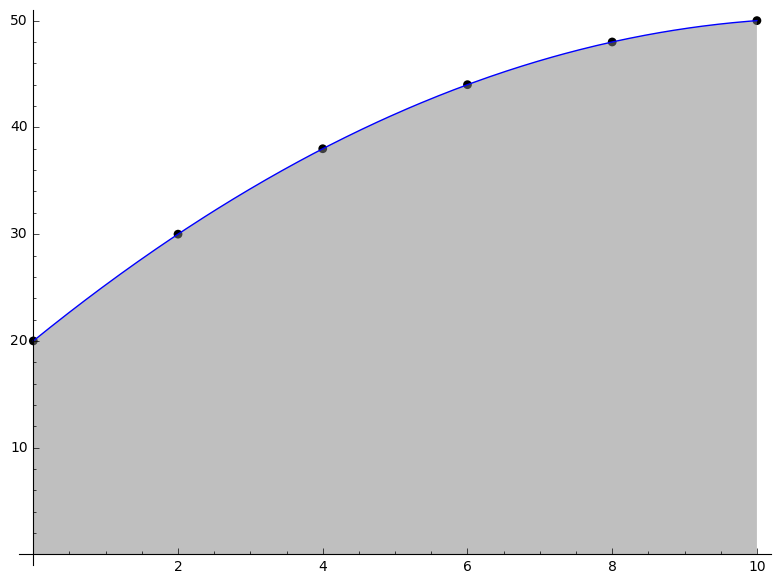
\includegraphics[scale=0.3]{nonlinearVelocity}
  \end{center}
\end{frame}

\begin{frame}{Generalizing our Analysis}
  When we use a Left-Hand Sum, we can't necessarily write down the error explicitly because the error isn't quite a triangle:
  \begin{center}
    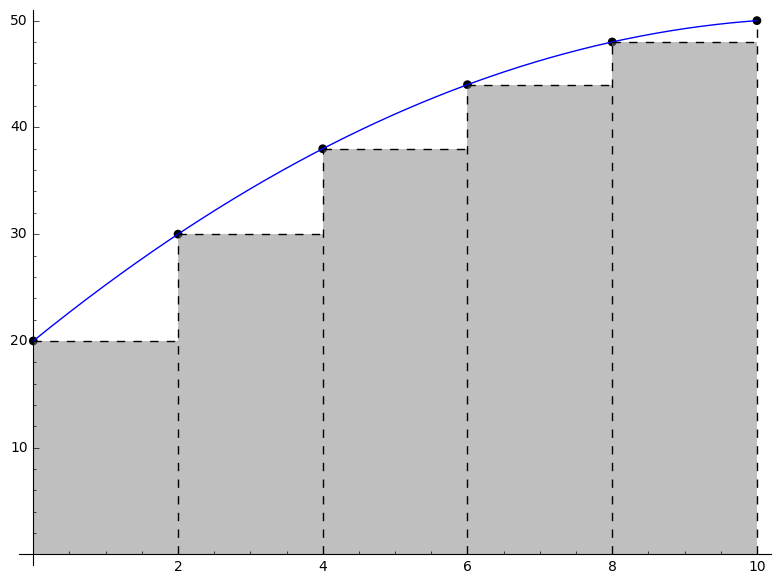
\includegraphics[scale=0.3]{nonlinearLeftSum}
  \end{center}
  \onslide<2->{However, we can use differential calculus to get around this.} 
\end{frame}

\begin{frame}{Linearization for Left-Hand Sums}
  Let $f$ be a continuous function.
  Recall that if we take $\Delta t$ sufficiently small, then we can use the Tangent Line Approximation,
  $$f(t) \approx f^\prime(a)(t - a) + f(a),$$
  to ensure that $f$ is basically a line whenever $a \leq t \leq a + \Delta t$.
\end{frame}

\begin{frame}{Linearization for Left-Hand Sums (Cont.)}
  Say we want to find the area beneath a continuous curve, $f$, on the interval $[a,b]$.
  \begin{itemize}
  \item<2->
    We can control the size of $\Delta t$ by increasing the number of points in a partition
    $$a = t_0 < t_1 < t_2 < \cdots < t_{n-1} < t_n = b$$
    since
    $$\Delta t = \frac{b - a}{n}.$$
  \item<3->
    This means that if we use enough points, 
    $$f(t) \approx f^\prime(t_i)(t - t_i) + f(t_i),$$
    whenever $t_i \leq t \leq t_{i+1}$, and in particular
    $$f(t_{i+1}) \approx f^\prime(t_i)\Delta t + f(t_i).$$
  \end{itemize}
\end{frame}

\begin{frame}{Linearization for Left-Hand Sums (Cont.)}
  Using this linearization, we get the following picture on $[t_i, t_{i+1}]$: 
  \onslide<2->{
    \begin{center}
      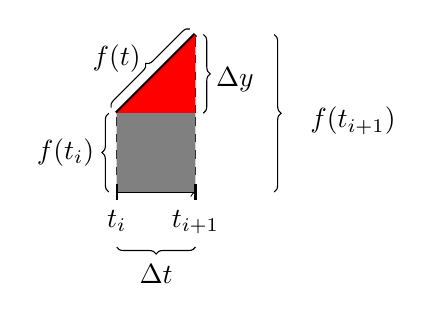
\begin{tikzpicture}
        \draw [->] (0,0) -- (1,0);
        \draw [-] [dashed](0,0) -- (0,1);
        \draw [-] [dashed] (1,0) -- (1,1);
        \draw [-] [ultra thick] (0,1) -- (1,2);
        \draw [-] [dashed] (1,1) -- (1,2);
        \draw [-] [dashed] (0,1) -- (1,1);
        \path [fill = red] (0,1) -- (1,2) -- (1,1) -- (0,1);
        \path [fill = gray] (0,0) -- (0,1) -- (1,1) -- (1,0) -- (0,0);
        \draw [
          decoration={
            brace,
            raise=0.1cm
          },
          decorate
        ]
        (0,0) -- (0,1) node[pos=.8,anchor=north,xshift=-.65cm]{$f(t_i)$};
        \draw [
          decoration={
            brace,
            mirror,
            raise=1cm
          },
          decorate
        ]
        (1,0) -- (1,2) node[pos=.6,anchor=north,xshift=2cm]{$f(t_{i+1})$};
        \draw [
          decoration={
            brace,
            mirror,
            raise=0.1cm
          },
          decorate
        ]
        (1,1) -- (1,2) node[align=center,pos=.7,anchor=north,xshift=.5cm]{$\Delta y$};
        \draw [
          decoration={
            brace,
            raise=0.1cm
          },
          decorate
        ]
        (0,1) -- (1,2) node[align=center,pos=1,anchor=north,xshift=-1cm]{$f(t)$};
        \draw [
          decoration={
            brace,
            mirror,
            raise=0.7cm
          },
          decorate
        ]
        (0,0) -- (1,0) node[pos=0.5,anchor=north,yshift=-.8cm]{$\Delta t$};
        \draw[thick] (0,-.1) node[below]{$t_i$} -- (0,0.1);
        \draw[thick] (1,-.1) node[below]{$t_{i+1}$} -- (1,0.1);
      \end{tikzpicture}
    \end{center}
  }
  \onslide<3->{
    By our previous analysis, the Left-Hand Sum underestimates the area under $f$ on the interval $[t_i, t_{i+1}]$ by approximately
  }
  $$\onslide<4->{\frac{1}{2}\Delta y \Delta t} \onslide<5->{= \frac{1}{2}\left[f(t_{i+1}) - f(t_i)\right]\Delta t.}$$
\end{frame}

\begin{frame}{Linearization for Left-Hand Sums (Cont.)}
  \begin{itemize}
  \item<1->
    By our work in Chapter 4, $f$ attains a global maximum, $M$, and a global minimum, $m$, on $[a,b]$. 
  \item<2->
    This means we can bound the approximate error of the {\bf underestimate} by
    $$\onslide<3->{\frac{1}{2}\left[f(t_{i+1}) - f(t_i)\right]\Delta t} \onslide<4->{ \leq \frac{1}{2}\left[M - m\right]\Delta t.}$$
  \item<5->
    Since $M - m$ is a fixed constant, this value goes to zero as $n$ becomes large!
  \item<6->
    This means we can compute the area under our curve to arbitrary precision by increasing the number of points in our partition.
  \item<7->
    As we increase the number of points in our partition, the Left-Hand Sum {\bf increases} towards the area under the curve.
  \end{itemize}
\end{frame}

\begin{frame}{Left Sum}
  \animategraphics[loop,controls,scale=0.3]{12}{leftEstimate/leftEstimate-}{0}{99}
\end{frame}

\begin{frame}{Linearization for Right-Hand Sums}
  \begin{itemize}
  \item<1->
    Just as in the linear case, the analysis of the Right-Hand Sums is completely symmetric.
  \item<2->
    After linearizing, the approximate error for the {\bf overestimate} is 
    $$\onslide<3->{\frac{1}{2}\left[f(t_{i+1}) - f(t_i)\right]\Delta t} \onslide<4->{ \leq \frac{1}{2}\left[M - m\right]\Delta t.}$$
  \item<5->
    Again, as $M - m$ is a constant, this value goes to zero as $n$ becomes large!
  \item<6->
    This means we can compute the area under our curve to arbitrary precision by increasing the number of points in our partition.
  \item<7->
    As we increase the number of points in our partition, the Right-Hand Sum {\bf decreases} towards the area under the curve.
  \end{itemize}
\end{frame}

\begin{frame}{Right Sum}
  \animategraphics[loop,controls,scale=0.3]{12}{rightEstimate/rightEstimate-}{0}{99}
\end{frame}

\subsection{Applying Our Method}
\begin{frame}{Our Distance Traveled Example}
  Recall that we started this excursion with the following question:\\
  \onslide<2->{
  \begin{minipage}[c]{\linewidth}
    \begin{center}
      Given the table of velocities and times\\
      \begin{tabular}{c||c|c|c|c|c|c}
        time (sec) & 0 & 2 & 4 & 6 & 8 & 10\\
        \hline
        speed (ft/sec) & 20 & 30 & 38 & 44 & 48 & 50\\
      \end{tabular}\\
    \end{center}
    can we determine how far the car traveled?
  \end{minipage}
  }
\end{frame}

\begin{frame}{Our Distance Traveled Example (Cont.)}
  It is possible to fit the data to the quadratic
  $$v(t) = \frac{-1}{4}t^2 + \frac{11}{2}t + 20.$$
  \onslide<2->{
    That is,
  \begin{center}
    \begin{tabular}{c||c|c|c|c|c|c}
      t & 0 & 2 & 4 & 6 & 8 & 10\\
      \hline
      f(t) & 20 & 30 & 38 & 44 & 48 & 50\\
    \end{tabular}
  \end{center}
  }
  \onslide<3->{
    This is the curve under which we've been attempting to estimate the area.
    }
  \onslide<4->{
    Later, we'll be able to explicitly compute that the area under this curve--which represents the distance traveled over those ten seconds--is
  $$\frac{1175}{3} = 391.\overline{6}\ \text{feet}$$
    }
\end{frame}

\begin{frame}{Our Distance Traveled Example (Cont.)}
  With 5 equidistant points
  \begin{itemize}
    \item<2->
      Our Left-Hand Sum estimated 360 feet,
    \item<3->
      Our Right-Hand Sum estimated 420 feet,
    \item<4->
      Our average estimated 390 feet, which was quite close.
  \end{itemize}
\end{frame}

\begin{frame}{Our Distance Traveled Example (Cont.)}
  Here is a table of Left-Hand Sums for $n+1$ points:
  \begin{center}
    \begin{tabular}{ll}
      $n$ & $\sum_{i=0}^{n-1}f(t_i)\Delta t$\\
      \hline
      \onslide<2->{10 & 376.25\\}
      \onslide<3->{100 & 390.1625\\}
      \onslide<4->{1,000 & 391.516625\\}
      \onslide<5->{10,000 & 391.65166625\\}
      \onslide<6->{100,000 & 391.6651666625\\}
    \end{tabular}
  \end{center}
  \onslide<7->{
    So we can see that as $n$ increases, the Left-Hand Sums increase towards the actual area under the curve, as expected.
  }
\end{frame}

\begin{frame}{Our Distance Traveled Example (Cont.)}
  Here is a table of Right-Hand Sums for $n+1$ points:
  \begin{center}
    \begin{tabular}{ll}
      $n$ & $\sum_{i=1}^{n}f(t_i)\Delta t$\\
      \hline
      \onslide<2->{10 & 406.25\\}
      \onslide<3->{100 & 393.1625\\}
      \onslide<4->{1,000 & 391.816625\\}
      \onslide<5->{10,000 & 391.68166625\\}
      \onslide<6->{100,000 & 391.6681666625\\}
    \end{tabular}
  \end{center}
  \onslide<7->{
    So we can see that as $n$ increases, the Right-Hand Sums decrease towards the actual area under the curve, as expected.
  }
\end{frame}
\end{document}
